%!TEX root = ../dissertation.tex
\begin{savequote}[75mm]
There are some things you learn best in calm, and some in storm.
\qauthor{Willa Cather}
\end{savequote}

\chapter{Apache Storm}

Apache Storm is a reliable, distributed and fault-tolerant system for stream processing.
The beginnings of the project were at Backtype (later bought by Twitter) and created by Nathan Marz.
He open sourced Storm on September the 19th in 2011. The project rapidly got a big development coummunity and
on September the 18, 2013 Nathan moved Storme to Apache Incubator.\\

Storm works with different types of components which are responsible for clear defined task.
This components are bundled and managed in a so called \textbf{Topology}.
The entrypoint and the stream input is handled by a \textbf{Spout}, the spout passes to \textbf{Bolts}.
Bolts are responsible for the main data processing and persists the data.
They can be chained or parallelised in a way that fits best for your current problem.

\begin{figure}[hp]
\centering
\captionsetup{justification=centering}
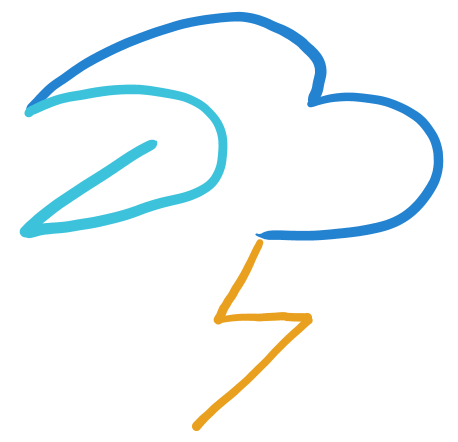
\includegraphics[width=100pt]{images/storm.png}
\caption[Storm]{Storm}
\end{figure}
\newpage

\section{Spout}


\newpage

\section{Bolt}

\newpage

\section{Topology}